\section{Apache RabbitMQ}
\subsection{Định nghĩa}
\begin{itemize}
 \item Rabbit MQ là một message broker mã nguồn mở thực thi chuẩn AMQP. 
 \item Message broker là một mô-đun chương trình trung gian có nhiệm vụ chuyển giao thức thông điệp chính thức từ bên gửi sang thông điệp chính thức của bên nhận.
\end{itemize}

\subsection{Các chuẩn giao thức mà RabbitMQ hỗ trợ}
\begin{itemize}
	\item Hỗ trợ chuẩn giao thức AMQP 0.9.1
	\item Ngoài ra RabbitMQ cũng hỗ trợ các giao thức của message queue khác qua các plugins:
	\begin{itemize}
		\item STOMP
		\item MQTT
		\item AMQP 1.0
	\end{itemize}
\end{itemize}

\subsection{Các định nghĩa}
\subsubsection{Queues}
\begin{figure}[h]
    \centering
    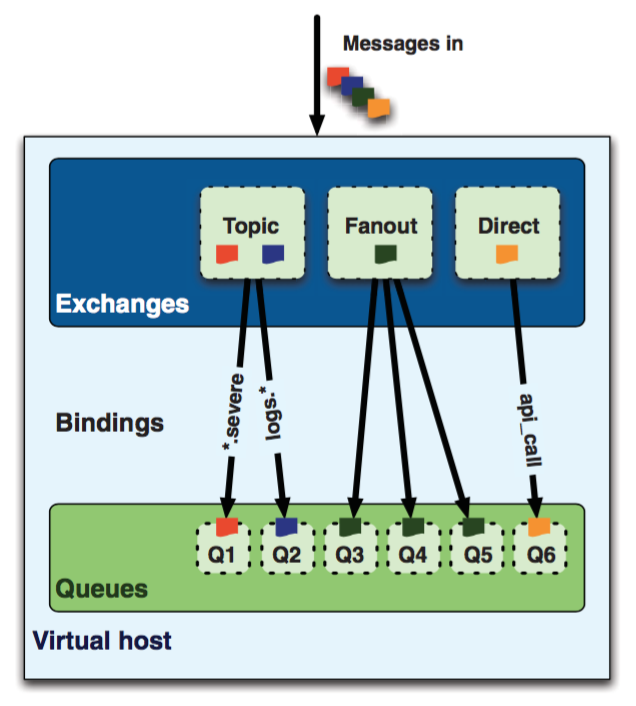
\includegraphics[width=0.3\textwidth]{amqp-stack}
    \caption{Amqp stacks: exchanges, Bindings and Queues}
    \label{fig:mesh1}
\end{figure}
Là nơi các message được chứa và chờ được các consumers nhận. Consumers có thể nhận các thông điệp từ queue theo một trong hai cách sau:
\begin{itemize}
	\item Đăng ký nhận thông qua lệnh basic.consume trong AMQP. Lệnh này sẽ tạo kênh (channel) đặt trong chế độ nhận đến khi nào huỷ đăng ký khỏi hàng đợi (queue). Khi subcribe vào một queue, consumber sẽ nhận tự động nhận các thông điệp nếu có từ queue sau khi xử lý xong thông điệp cuối cùng trong queue. Nên sử dụng basic.consume trong trường hợp consumser xử lý nhiều thông điệp một cách tự động ngay sau khi thông điệp này được chuyển tới queue.
	\item Đôi khi chỉ cần có một tin nhắc duy nhất từ hàng đợi mà không yêu cầu phải liên tục, sử dụng lệnh basic.get. 	
\end{itemize}
Nếu có nhiều consumers đăng ký vào cùng một hàng đợi, RabbitMQ sẽ chỉ chuyển thông điệp đến cho một hàng đợi theo cơ chế round-robin. 
\newline
Nếu sử dụng cơ chế auto-ack, thì khi consumer nhận được thông điệp từ queue sẽ phải gửi lại cho RabbitMQ một acknowledge message để  RabbitMQ biết là thông điệp đó đã được nhận và remove khỏi queue. Trong trường hợp consumer nhận thông điệp và mất kết nối tới RabbitMQ, RabbitMQ sẽ coi thông điệp đó vẫn chưa được gửi đi và sẽ vẫn lưu lại ở queue để phân phát cho consumer mới đăng ký.
\newline
Một số thuộc tính hay dùng cho queue:
\begin{itemize}
	\item exclusive: nếu set là true thì queue là private, chỉ được consume bởi một ứng dụng duy nhất. Nên dùng khi muốn hạn chế một queue chỉ được duy nhất một consumer.
	\item auto-delete: queue sẽ tự động delete khi queue không có consumer nào đăng ký nhận message. Nếu cần một queue tạm để cho duy nhất một consumer có thể kết hợp exclusive và auto-delete.
\end{itemize}

\subsubsection{Exhanges và bindings}
Bất cứ khi nào bạn muốn phân phát message tới queue, thì phải gửi message vào một exchange. Một queue sẽ được gắn (binding) vào exchange bởi một routing key. Exchange sẽ dựa vào routing-key để quyết định queue nào sẽ được phân phát message. \\
Các loại exchange:
\begin{figure}[h]
    \centering
    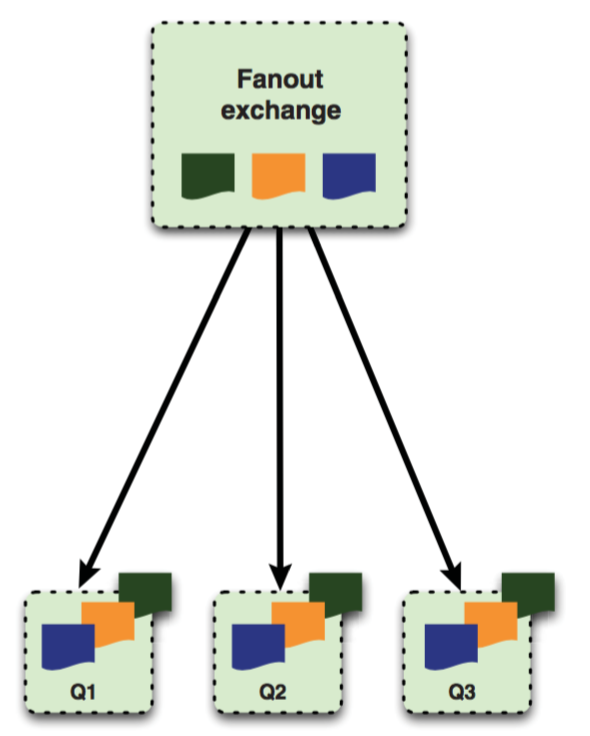
\includegraphics[width=0.3\textwidth]{fanout-exchange}
    \caption{Fanout exchange message flow}
    \label{fig:mesh1}
\end{figure}

\begin{figure}[h]
    \centering
    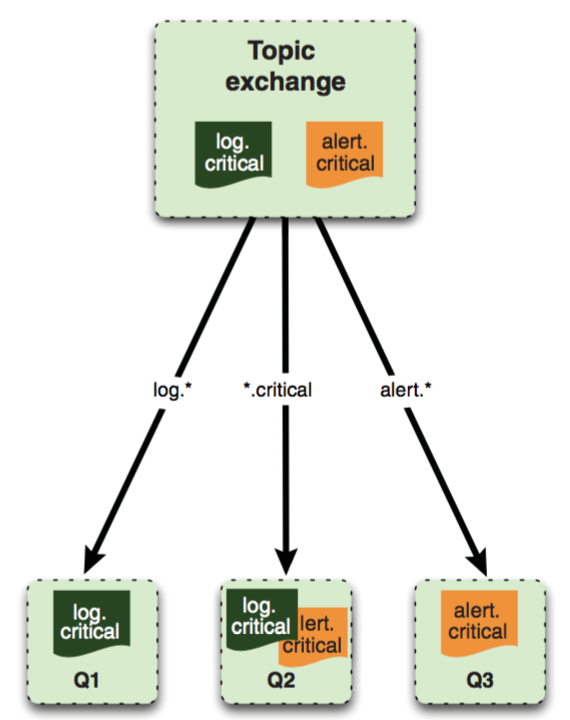
\includegraphics[width=0.3\textwidth]{topic-exchange}
    \caption{Topic exchange message flow}
    \label{fig:mesh1}
\end{figure}
